\section{Opis wybranych baz danych}

W tym rozdziale przedstawione zostały opisy wybranych baz danych dla systemu iOS: Core Data, Realm, FMDB oraz User Defaults. W systemie iOS istnieje wiele rozwiązań umożliwiających wdrożenie bazy danych w aplikacji, przedstawione tutaj przykłady są jednymi z najczęściej stosowanych przez programistów bazami danych w aplikacjach iOS.

\subsection{SQLite}
SQLite jest wewnątrz procesową biblioteką dostępną w systemie iOS. Kod opisywanej bazy jest dostępny publicznie, można go używać w dowolnym celu komercyjnym lub prywatnym bez żadnych opłat. Sprawia to że baza ta jest jednym z najczęściej wybieranych przez programistów rozwiązań do przechowywania danych w aplikacjach. Wybór tej biblioteki jest też kierowany tym iż projekt istnieje już od 2000 roku a jego twórcy deklarują wsparcie aż do 2050 roku\cite{SQLite-doc} .\par

SQLite jest ""lżejszą" wersją SQL więc korzystanie z funkcji biblioteki zostało znacząco uproszczone. Baza ta nie posiada wydzielonych procesów serwerowych, dane zapisuje i odczytuje ze zwykłych plików dyskowych. Kompletna baza danych programu zawierająca wszystkie tabele, relacje i tym podobne komponenty zapewniające poprawne działanie bazy przechowywane są w jednym pliku na dysku. Dzięki przechowywaniu wszystkich tych informacji w jednym pliku, informacje te mogą być kopiowane w stanie nienaruszonym pomiędzy programami.\par

System iOS zapewnia wbudowaną obsługę baz SQLite, nie istnieje więc potrzeba dodawania do projektu dodatkowych bibliotek. Cała komunikacja z biblioteką jest natywna i wymaga jedynie zaimportowania SQLite3. 
SQLite jest bazą relacyjna i zapewnia dodawanie relacji pomiędzy tabelami takich jak: 

\begin{itemize}
  \item N:M – wiele do wielu
  \item 1:N – jeden do wielu
  \item 1:1 – jeden do jednego 
\end{itemize}

Zapewniona została też obsługa danych takich jak: 

\begin{itemize}
	\item NULL - wartość pusta
	\item INTEGER - wartość całkowita ze znakiem, przechowywana w 1, 2, 3, 4, 6 lub 8 bajtach w zależności od wielkości wartości
	\item REAL - wartość zmiennoprzecinkowa, przechowywana jako 8-bajtowa liczba zmiennoprzecinkowa IEEE
	\item TEXT - wartością jest ciąg znaków przechowywany przy użyciu kodowania bazy danych (UTF-8, UTF-16)
	\item BLOB - wartość przeznaczona do przechowywania wielkich plików w formie bajtowej takich jak obrazy, muzyka itp. 
\end{itemize}

SQLite nie zapewnia wsparcia dla przechowywania obiektów zawierających datę. W celu zapisania daty w tablicy należy używać wartości tekstowych lub liczbowych a następnie zapewnić ich odpowiednie odczytanie i konwersje do odpowiednich obiektów języka w którym przebiega implementacja programu. 

\subsection{Core Data}

Core Data jest dedykowanym rozwiązaniem Apple umożliwiającym zaimplementowanie bazy danych w aplikacjach iOS i MacOS. Została wprowadzona od wersji iOS 3.0 w 2009 roku. Znacznie szybciej istniała możliwość używania tej bazy danych w MacOS,  pierwszą wersją systemu która to umożliwiła był MacOS Tiger, który ukazał się w 2005 roku.\par

Mimo że Core Data służy do przechowywania danych sama w sobie nie jest bazą danych a framework-iem który zarządza diagramem obiektów aplikacji. Diagram obiektów jest to zbiór obiektów powiązanych ze sobą relacjami. Core Data zajmuje się zarządzaniem cyklem życia obiektów w diagramie obiektów na dysku a także oferuje interfejs do przeszukiwania obiektów, którymi zarządza. Core Data daje także możliwość sprawdzania poprawności danych wejściowych, modelowania modeli danych czy też śledzenia zmian. \par

Core Data jako rozwiązanie implementacji bazy danych korzysta z SQLite, przechowuje za jego pomocą wszystkie obiekty na dysku. Rozszerza jednak oferowane funkcjonalności SQLite o obsługę bazy w kilku wątkach, tworzenia tymczasowych obiektów (kiedy nie jesteśmy pewni, czy one zostaną zapisane na dysk), automatycznie nasłuchiwanie na zmiany w bazie danych, między innymi jeśli wyświetlamy dane użytkownika na ekranie, a dane w bazie danych się zmienią (za sprawą na przykład drugiego wątku pracującego z zewnętrznym serwerem API) to dostaniemy odpowiednie powiadomienie. Core Data zapewnia łatwą integracje z kontrolkami interfejsu użytkownika takimi jak UITableView (kontrolka odpowiedzialna za wyświetlanie tabel/list) między innymi zapewniając automatyczne tworzenie indeksów i sekcji.\par

Core Data jest zorganizowana w dużą hierarchie klas, lecz używane są najczęściej podstawowe obiekty takie jak: 

\begin{itemize}
	\item NSManagedObject - Klasa reprezentująca jeden wiersz tabeli, zapewniajacy dostęp do danych przechowywanych w wierszu.
	\item NSManagedObjectContext - Główny kontekst bazy, wykonuje operacje na bazie. Pozwala na zapis aktualnego stanu bazy danych.
	\item NSManagedObjectModel	- Klasa reprezentujący model tablicy. 
	\item NSFetchRequest - Klasa pozwalająca utworzyć zapytanie mające na celu przeprowadzenie operacji na danych.
	\item NSPersistentStoreCoordinator - Klasa odpowiedzialna za operacje na pliku który przechowuje dane bazy. Za pomocą tej klasy możliwe jest całkowite jest usunięcie. 
	\item NSPredicate - Klasa za pomocą której tworzymu zapytanie do bazy danych, używana jest jako parametr metody klasy NSFetchRequest.
\end{itemize}

Tak samo jak poprzednio opisywana baza danych Core Data pozwala na tworzenie wszystkich możliwych relacji pomiędzy tabelami. Framework zapewnia też możliwość przechowywania w tabeli wielu typów danych takich jak: 

\begin{itemize}
	\item String - łańcuch znaków
	\item Int - liczba całkowita
	\item Float - liczba zmiennoprzecinkowa
	\item Double  - liczba zmiennoprzecinkowa
	\item Boolean - wartość boolowaska prawda/fałsz 
	\item Date - obiekt przechowujący date
	\item Binary Data - dane w formacie binarnym 
	\item URI - adresy zasobów
	\item Transformable - wartość do przechowywana niestandardowych danych 
\end{itemize}

Jedną z ważnych cech tej bazy danych jest możliwość graficznego definiowania schematu bazy, pełne wsparcie zapewnia środowisko programistyczne XCode. Na rysunku  poniżej został przedstawiony edytor bazy danych. \par

\begin{figure}[h]
	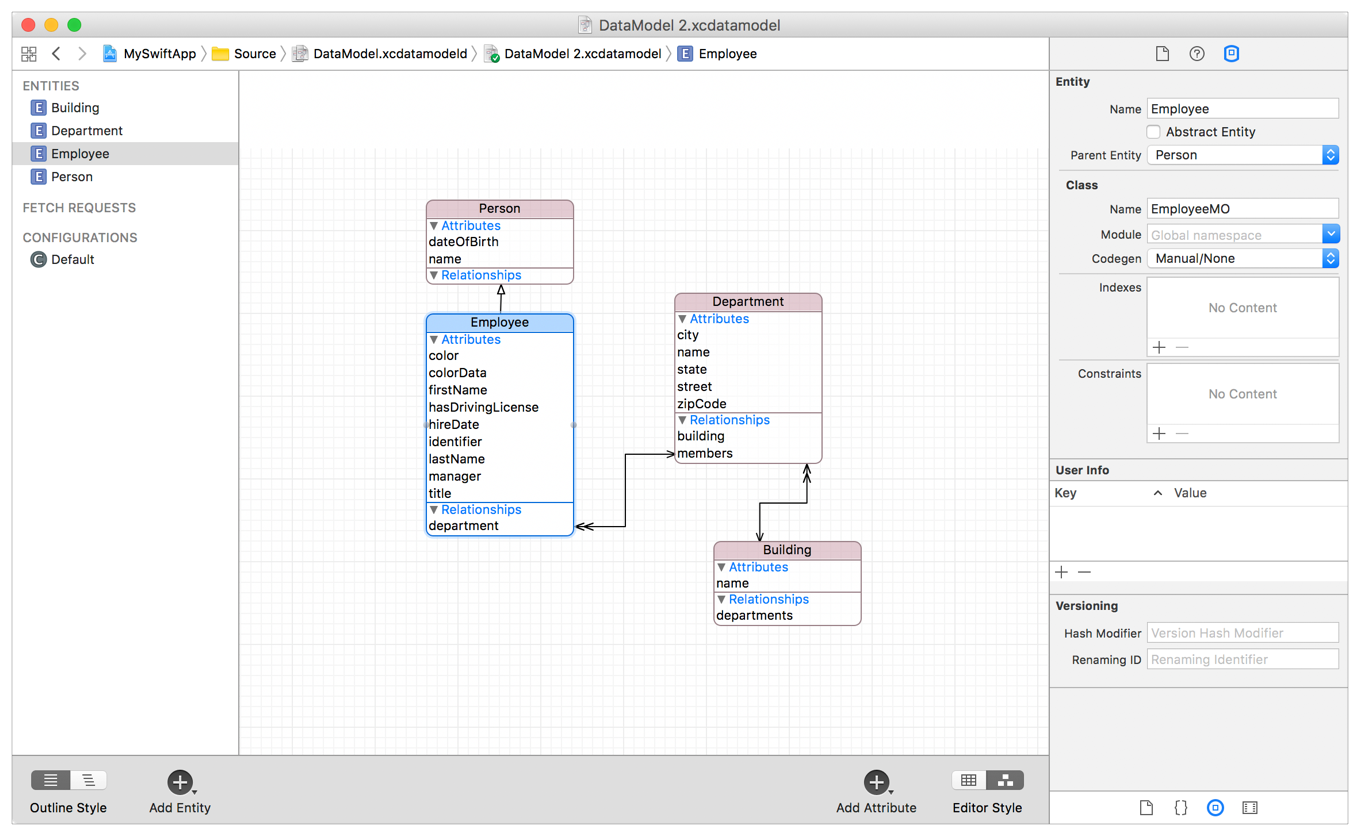
\includegraphics[width=\linewidth]{img/Entity_Inheritence_2_2x.png}
	\caption{Edytor Core Data w XCode}
	\label{fig: CoreDataEdytor}
\end{figure}

Dodatkowo XCode pozwala generować klasy dla obiektów stworzonych za pomocą edytora, które wykorzystywane są później do tworzenia obiektów przed zapisem do bazy. Istnieją też inne narzędzia, które umożliwiają wygenerowanie klas dla stworzonego diagramu. Jednym z najpopularniejszym jest Mogenerator. Zapewnia on wsparcie dla języka Swift i Objective -C.

\newpage
\subsection{FMDB}

FMDB jest biblioteką opakowującą SQLite. Można więc stwierdzić że FMDB i SQLite służą temu samemu celowi - umożliwiają efektywne zarządzanie danymi aplikacji. Lecz sposoby w jaki się je używa znacząco się od siebie różnią. FMBD oferuje interfejs wyższego poziomu ukrywając wszystkie szczegóły SQL takie jak połączenie i komunikacja z bazą, ale  dalej oferuje dokładną obsługę danych. \par 
FMDB zapewnia funkcje SQLite więc podczas implementacji nie trzeba zajmować się połączeniami a także pisaniem i odczytywaniem danych do i z bazy. Biblioteka ta jest dobrym rozwiązaniem dla programistów, którzy chcą wykorzystać swoją wiedzę SQL i pisać własne zapytania, ale bez potrzeby pisania własnego menadżera SQLite. FMDB działa w dwóch językach: Swift i Objective-C oraz bardzo szybko integruję się z projektem iOS. Jej twórcy zapewniają, że jest ona zaimplementowana tak aby zapewnić najwyższą wydajność SQLite, lepszą od prostych implementacji menadżerów dla SQLite. \par

Biblioteka jest bardo prosta w użyciu. Możemy w niej wyróżnić trzy główne klasy: 

\begin{itemize}
	\item  FMDatabase - Reprezentuje pojedynczy obiekt bazy danych. Używana jest do wykonywania instrukcji SQL. 
	\item FMResultSet - Klasa przetrzymująca rezultaty zapytań SQL wykonanych na bazie danych.
	\item FMDatabaseQueue - Klasa która jest używana podczas wykonywania kwerend i aktualizacji danych w bazie przy użyciu wielu wątków.
\end{itemize}

Jako, że FMBD oferuje interfejs wyższego poziomu do SQLite dodana została obsługa typów danych takich jak: 

\begin{itemize}
	\item Bool -  wartość boolowaska prawda/fałsz 
	\item Date - obiekt przechowujący date
\end{itemize}

Obsługa tych dwóch typów danych wymagała w SQLite dodatkowych operacji. W przypadku wartości prawda/fałsz należało zapisywać w tabeli zero lub jeden i odpowiednio konwertować wartości liczbowe do wartości Bool. Sytuacja podczas zapisu daty w SQLite wygląda podobnie, należy najpierw wartość daty skonwertować do wartości tekstowej a podczas odczytu danych wartość tekstową skonwertować do obiektu przechowującego datę. FMBD w znaczącym stopniu ułatwia obsługę tak często używanych w bazach danych wartości. Dodatkowo warto wspomnieć iż FMDB będąc biblioteką opakowującą SQLite daje możliwość korzystania z dokumentacji SQLite, która jest bardzo dokładna i ciągle rozwijana. Trudno więc zaprzeczyć, że biblioteka ta stanowi dobre rozwiązanie zastępujące standardowy SQLite. 

\subsection{Realm}

Realm różni się od poprzednio opisywanych baz SQL. Biblioteka ta jest obiektową bazą danych NoSQL. Przechowuje dane w postaci obiektów. Realm jest rozwiązaniem open-source więc jest w pełni darmową baza danych, dedykowaną do aplikacji mobilnych. Dodatkowo jest dostępna na systemy Android i iOS, co znacząco ułatwia prace nad aplikacjami dostępnymi nie tylko na jedną platformę. Współpracuje z projektami pisanymi w: Swift, Objective-C, Java, React Native, Xamarin i innymi. Biblioteka ujrzała światło dzienne w 2016 roku a pierwsza stabilna wersja wydana została w styczniu 2017 roku. Jedną z wyróżniających ją funkcji jest możliwość dwukierunkowej synchronizacji pomiędzy bazą serwera a bazą aplikacji.\par 

Realm swoją popularność zyskał poprzez szybkość, łatwość integracji z projektem oraz łatwością posługiwania się nim. Od bibliotek opakowujących SQLite oraz całego framework-u Core Data odróżnia go to, że większość typowych funkcji, takich jak odpytywanie bazy danych składa się z pojedynczych linii kodu. Dzięki temu używając biblioteki Realm uzyskuje się bardziej zwięzły kod i poprawia się jego czytelność. Podczas używania Realm nie potrzebna jest dobra znajomość SQL do zarządzania bazą i tworzenia zapytań. Nie wymagana jest też dobra znajomość Core Data, która jest zaawansowanym narzędziem i nie wiele osób posiada umiejętności pozwalające wydaje zarządzać tą bazą danych. W Realm dane są przechowywane jako obiekty dzięki czemu przy odczytywaniu czy zapisywaniu danych w bazie nie ma potrzeby stosowania żadnej biblioteki ORM (Object Relation Mapping) pozwalającej na konwersje danych pomiędzy obiektem programu a rekordem tabeli. Dzięki temu unikane są problemy z wydajnością dodatkowych bibliotek ORM. Interfejs biblioteki ogranicza się do trzech klas: 

\begin{itemize}
	\item Realm -  Główna klasa, pozwalająca na dostęp do bazy i wykonywanie operacji zapisu/odczytu.
	\item Object - Klasa reprezentująca model danych bazy.
	\item Result - Obiekt reprezentujący listę dane odczytane z bazy przy użyciu zapytania.
\end{itemize}
 \par

Realm tak jak Core Data czy FMDB zapewnia wsparcie dla wszystkich typów danych. Na uwagę zasługują tutaj relacje pomiędzy tabelami. Biblioteka jest obiektową bazą danych, nie ma więc w niej tabel i zwykłych relacji pomiędzy nimi. W Realm relacje pomiędzy obiektami tworzone są za pomocą linkowana obiektów. Każdy link tworzy link zwrotny jako relację odwrotną do dowolnego obiektu łączącego się z bieżącym obiektem obiektem. Za pomocą Reaml Studio możliwe jest także stworzenie pliku bazy danych na podstawie dokumentu CSV.  \par 

Dodatkowo Realm dostarcza również narzędzie Realm Studio widoczne na rysunku 2.2. Pozwala ono na łatwe zarządzanie bazą danych. Umożliwia otwieranie, przeglądanie i edytowanie lokalnych plików Realm.  

\begin{figure}[h]
	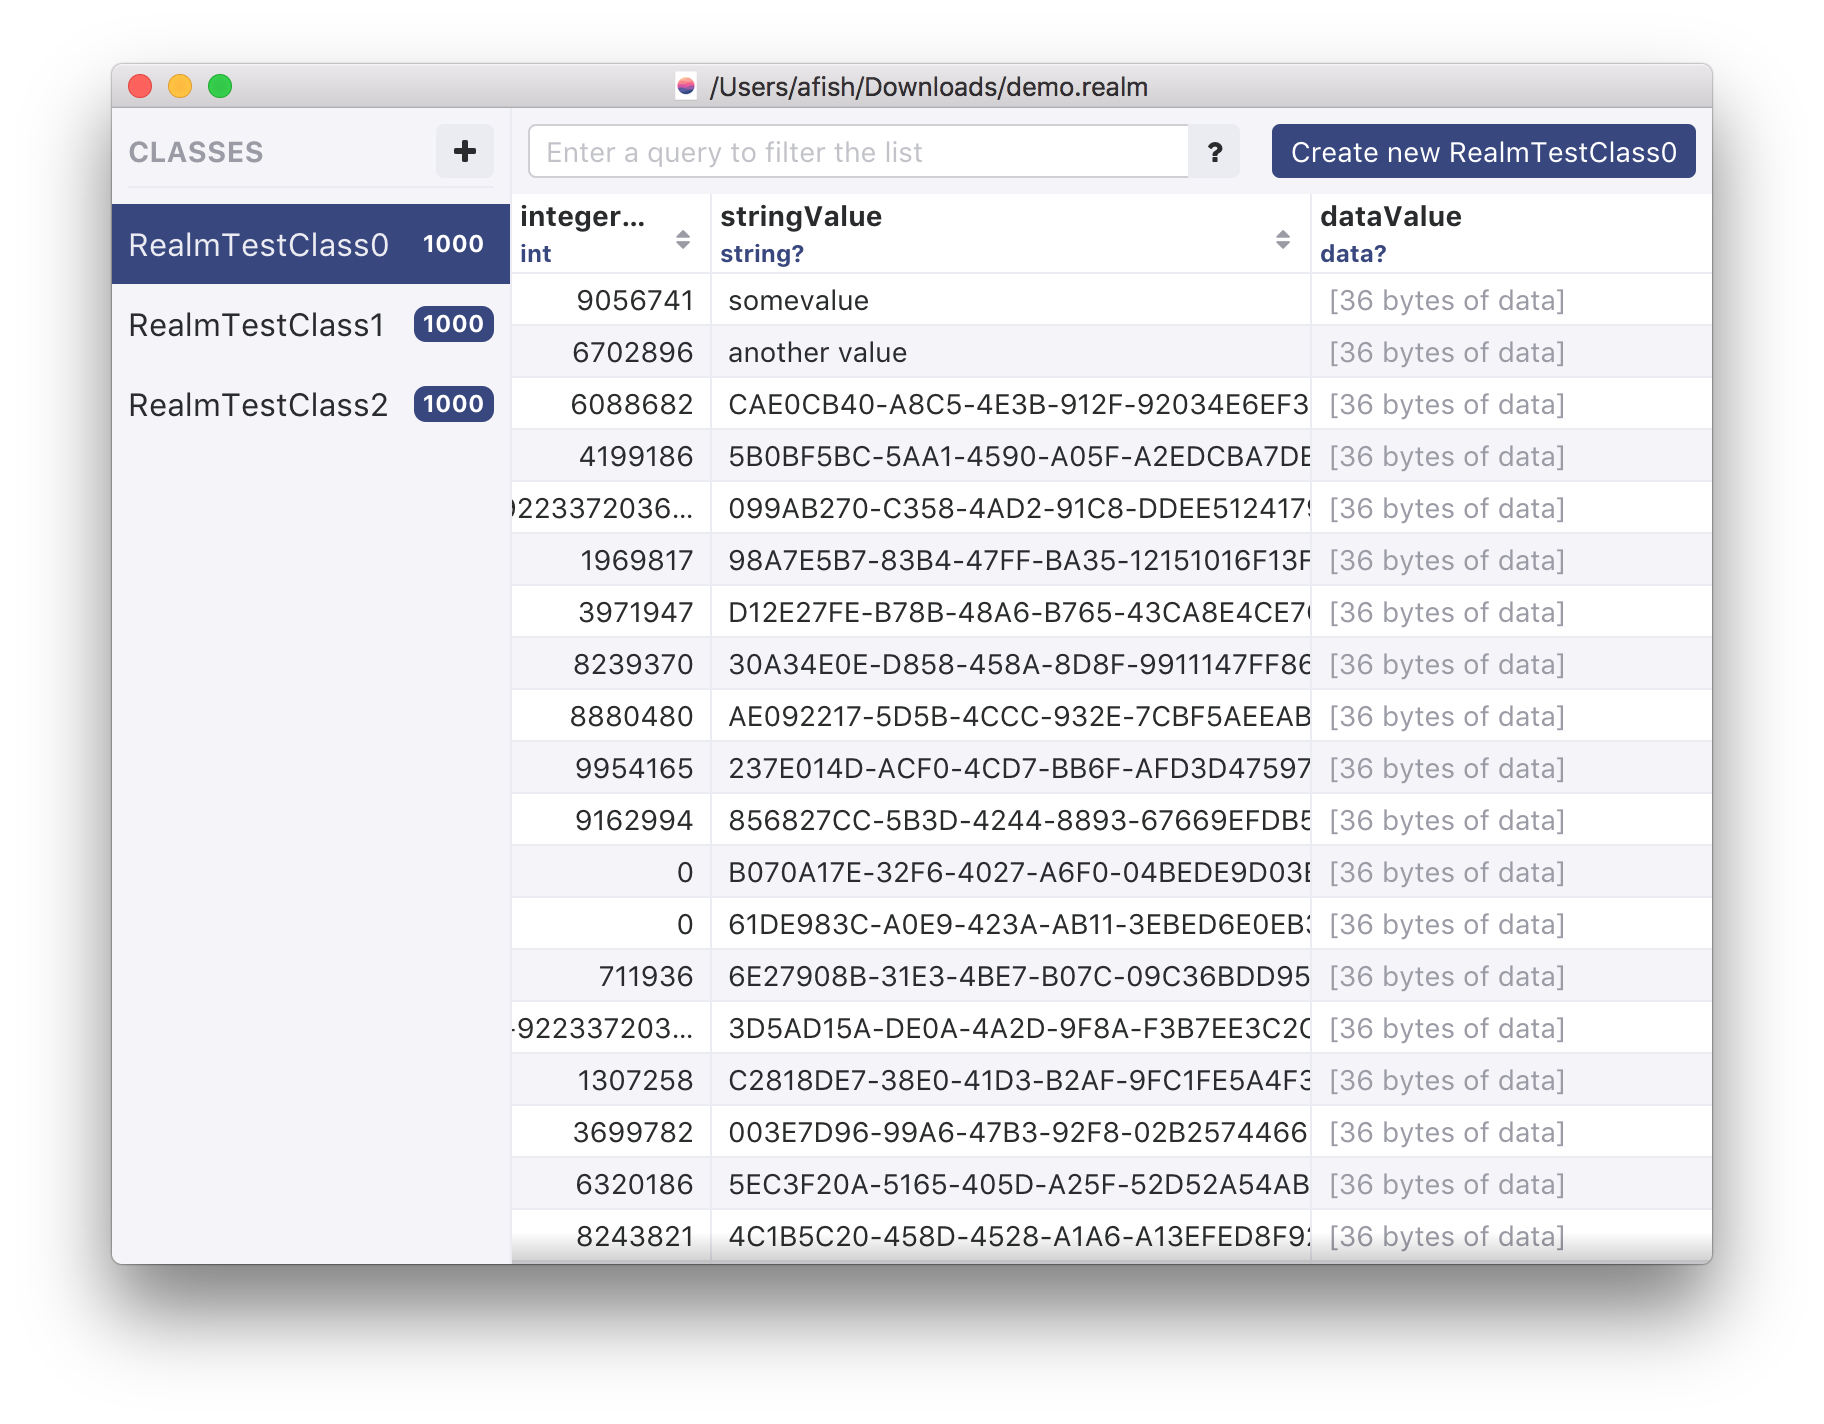
\includegraphics[width=\linewidth]{img/RealmStudio.png}
	\caption{Narzędzie Realm Studio}
	\label{fig: RealmStudio}
\end{figure}

\subsection{User Defaults}

Kolejnym z rozwiązań pozwalającym zapisywać i przechowywać dane w systemi iOS jest User Defaults - domyślna baza użytkownika. Dane w niej przechowywane są pary klucz - wartość. System pomimo iż nie jest prawdziwą bazą danych a jedynie interfejsem, który pozwala na przechowywanie potrzebnych, niewielkich danych aplikacji, został wybrany w tej pracy do porównania ponieważ wielu programistów używa go zamiast innych rozwiązań bazodanowych. Rozwiązanie to jest szybkie w implementacji i pozwala zapisywać niestandardowe obiekty jeżeli implementują protokół NSCoding i zostaną skonwertowane do prostej formy Data. Więcej informacji na temat sposobu zapisu i konwersji danych znajduję się w rozdziale ??. \par
  
User Defaults pozwala zapisywać wartości takie jak: Bool, Integer, Float, Double, String, Data, URL, Array, Dictionary. Zapis danych wykonuje się za pomocą funkcji set(:forKey:) a odczyt value(forKey:). 
